\documentclass[11pt,twoside]{report}

\usepackage[utf8]{inputenc}
\usepackage{graphicx}
\usepackage{bm}
\usepackage{amsmath}
\usepackage{amssymb}
\usepackage{mathtools}
\usepackage{caption}
\usepackage{subcaption}
\usepackage{geometry}

\newcommand{\defeq}{\vcentcolon=}

% Parentheses
\newcommand{\lk}{\left\langle}
\newcommand{\rk}{\right\rangle}
\newcommand{\lb}{\left\lbrace}
\newcommand{\rb}{\right\rbrace}
\newcommand{\lp}{\left(}
\newcommand{\rp}{\right)}
\newcommand{\ls}{\left[}
\newcommand{\rs}{\right]}


\graphicspath{{figures/}}

\geometry{
	a4paper,
%	showframe,
	twoside,
	includeall,
	top=15mm,left=30mm,right=10mm,bottom=15mm,
	marginparwidth=20mm,marginparsep=5mm
}

\begin{document}
\title{
	{LB with Oldroyd-B Report}\\
	{Institute for Computational Physics}\\
	{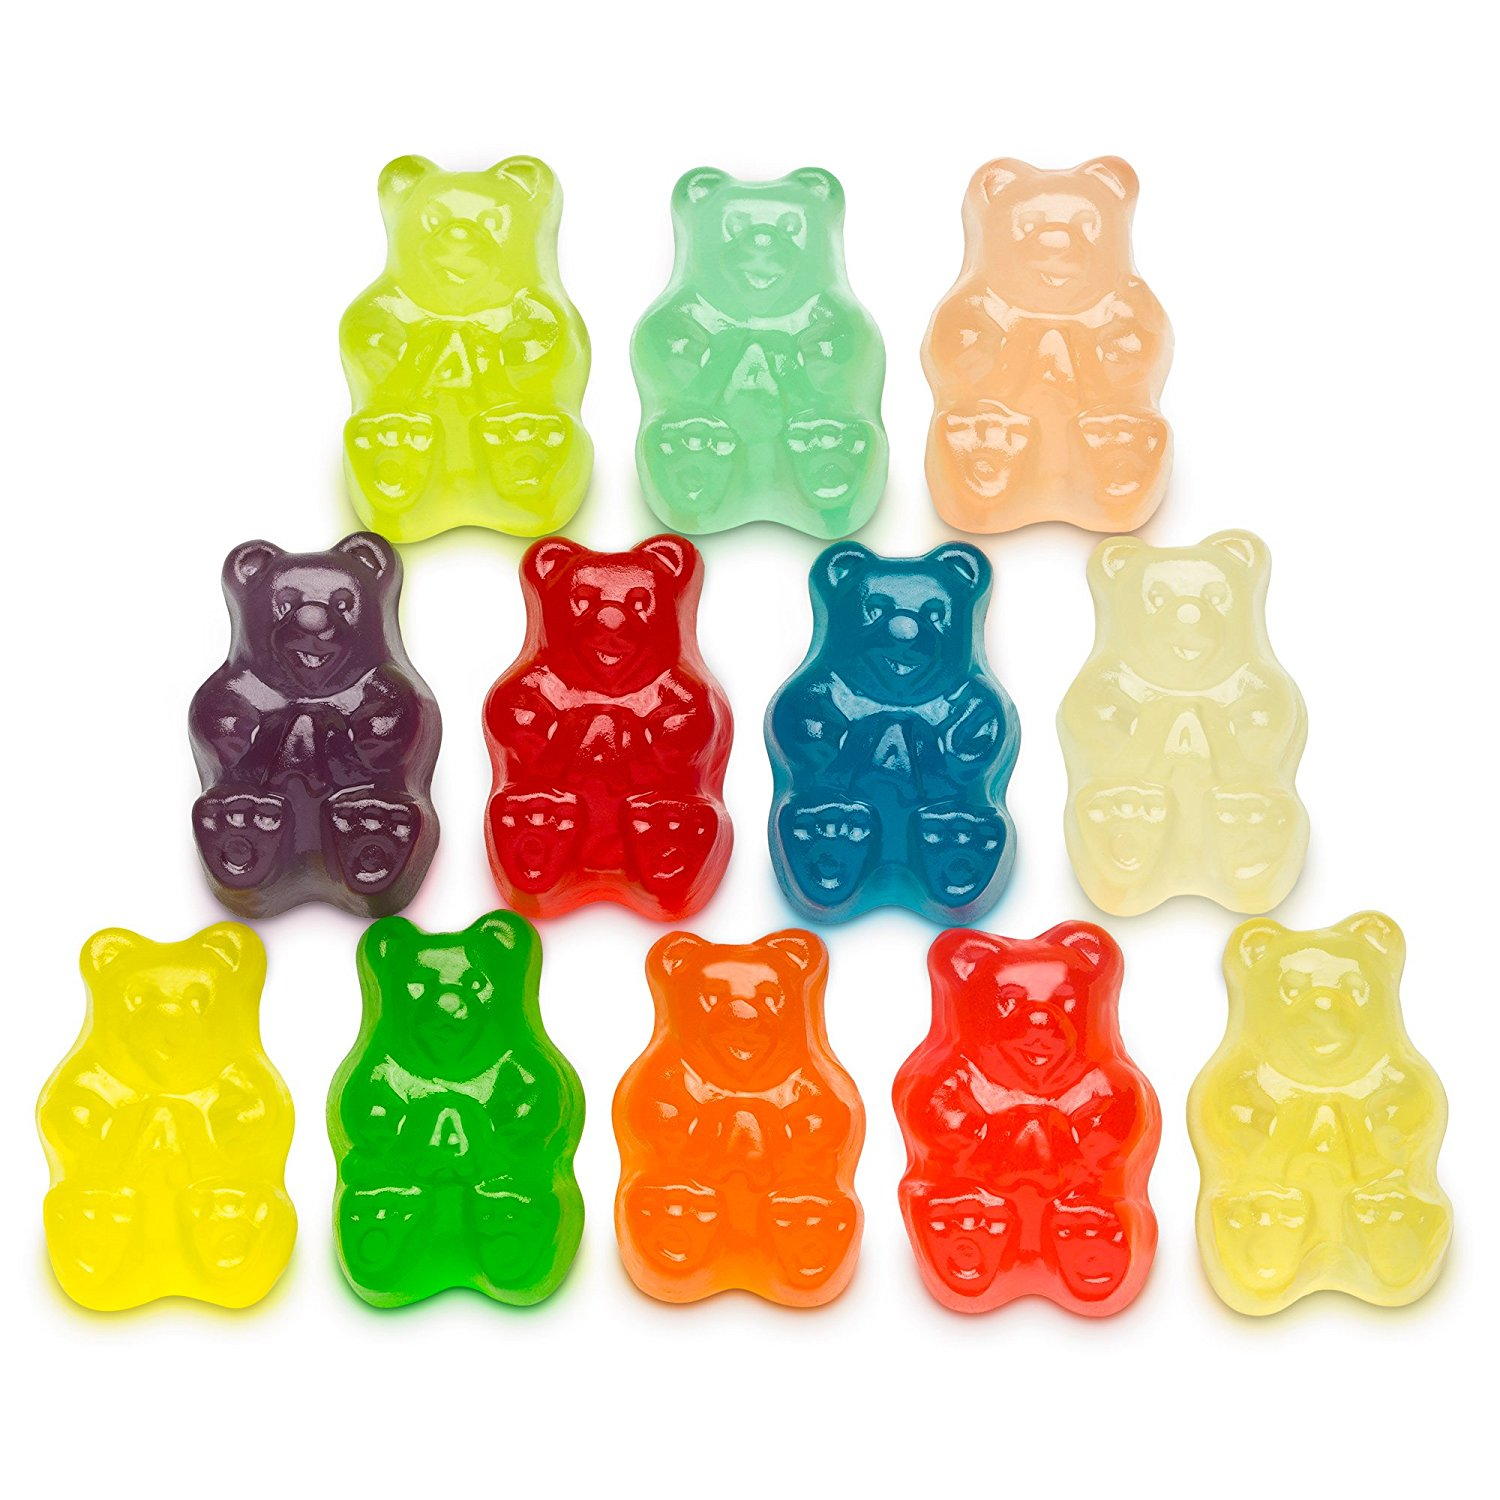
\includegraphics[width=0.8\textwidth]{title.jpg}}
}
\author{Cameron Nash Stewart}
\date{\today}
\maketitle

\chapter*{Dedication}
This work is dedicated to Haribo for supplying me with enough sugar to study physics and for inspiring me to delve into the fascinating world of complex fluids.

%\chapter{Introduction}
\chapter{Mathematical Model}
In this work we treat the solvent of a viscoelastic fluid as an incompressible fluid with the usual Navier-Stokes momentum and mass conservation equations. These are given by
\begin{equation}\label{eq:momentum_conservation}
\rho \left( \frac{\partial \bm{u}}{\partial t} + \left(\bm{u} \cdot \nabla\right)\bm{u}\right) =
-\nabla p +\eta_s \nabla^2 \bm{u} + \bm{F}^{\mathrm{ext}} + \nabla \cdot \bm{\tau} 
\end{equation}
and
\begin{equation}\label{eq:mass_conservation}
\nabla \cdot \bm{u} = 0,
\end{equation}
where $\rho$ is the density, $\bm{u}$ is the velocity field, $p$ is the pressure, $\eta_s$ is the viscosity of the solvent, $\bm{F}^{\mathrm{ext}}$ is an external force density on the fluid, and $\bm{\tau}$ the so-called extra stress tensor. Here we see that the divergence of the extra stress tensor leads to a forcing term in the momentum conservation equation. 

Although, on the microscopic level, viscoelastic effects are due to the stretching and relaxation of polymers suspended in the solvent, we will be using a continuum model to develop this extra stress tensor in time. The Oldroyd-B model is commonly used to describe viscoelastic flow and is mathematically equivalent to a fluid filled with harmonic spring "dumbells." The Oldroyd-B model provides a constitutive equation for the extra stress tensor which has the form
\begin{equation}\label{eq:short_oldroyd_b}
\overset{\nabla}{\bm{\tau}} = \frac{1}{\lambda_p}\left(2\eta_p\bm{d}- \bm{\tau}\right)
\end{equation}
where $\lambda_p$ and $\eta_p$ are the relaxation time and added viscosity of the polymer solution, respectively, and  
\begin{equation}\label{eq:rate_of_strain}
\bm{d} \defeq \frac{1}{2}\left(\nabla\bm{u} + \nabla \bm{u}^T\right)
\end{equation}
is the rate of strain tensor where $T$ indicates the transpose. The upper-convected time derivative is defined as
\begin{equation}\label{eq:upper_convected_derivative}
\overset{\nabla}{\bm{\tau}} \defeq \frac{\partial \bm{\tau}}{\partial t} + (\bm{u} \cdot \nabla)\bm{\tau} - \bm{\tau} \cdot \nabla\bm{u} -(\nabla\bm{u})^\intercal \cdot \bm{\tau}
\end{equation}
and describes the time evolution of a tensor being transported along a velocity field $\bm{u}$. Use of this time derivative is required so that our constitutive relation Note that it is important that we choose the convention that
\begin{equation}\label{eq:gradient_convention}
(\nabla \bm{u})_{\alpha\beta} \defeq \frac{\partial u_{\beta}}{\partial x_\alpha}
\end{equation}
in order that Eq.~\eqref{eq:upper_convected_derivative} be the correct form. Finally, we may write the constitutive equation as
\begin{equation}\label{eq:full_oldroyd_b}
\frac{\partial \bm{\tau}}{\partial t} + (\bm{u} \cdot \nabla)\bm{\tau}= \left(\bm{\tau} \cdot \nabla\bm{u} +(\nabla\bm{u})^T \cdot \bm{\tau}\right) + \frac{1}{\lambda_p}\left(2\eta_p \bm{d} - \bm{\tau}\right).
\end{equation}
We aim to develop these two equations numerically in order to simulate an Oldroyd-B fluid.
\chapter{Algorithm}
As described before, in order to simulate the viscoelastic fluid we must develop both the Navier-Stokes equations for the solvent simultaneously with the Oldroyd-B constitutive equation. In order to simulate the solvent we will use the Lattice-Boltzmann method, a standard Navier-Stokes solver that can easily be extended to apply the additional elastic force. We treat the development of the extra-stress tensor using a simple Euler-like scheme where the Lattice-Boltzmann method allows us a nice way to calculate the advection.
\section{The Lattice-Boltzmann Method}
Rather than directly discretize the Navier-Stokes equations, we will discretize the Boltzmann transport equation (BTE). It can be shown that solving the BTE is equivalent to solving the former. The Boltzmann equation describes the time development of the single particle distribution function in phase space and is given by
\begin{equation}\label{eq:boltzmann_transport}
\frac{d}{dt} f(\bm{x}, \bm{v}, t) = \frac{\partial f}{\partial t} + \bm{v} \cdot \nabla_{\bm{x}}f + \frac{\bm{F}}{m} \cdot \nabla_{\bm{v}} f =\Omega[f] 
\end{equation}
where $f$ is the single particle distribution function, $\bm{x}$ is position, $\bm{p}$ is momentum, $\bm{F}$ is force, and $\Omega[f]$ is the so-called collision operator. 

The collision operator contains information on how the disribution function changes due to particle-particle interactions and would be impossible to model directly. However, any collision operator we can dream up that conserves mass and momentum will allow us to convert the BTE into the Navier-Stokes equations. The simple choice we will use is known as the single relaxation time (SRT) operator and is given by
\begin{equation}\label{eq:single_relaxation_time}
\Omega[f] = \frac{1}{\lambda}\left(f^{\mathrm{eq}}(\bm{x}, \bm{v}) - f(\bm{x}, \bm{v}, t)\right)
\end{equation}
where $f^{\mathrm{eq}}$ is the single particle distribution function at equilibrium. Finally we arrive at the Boltzmann equation with SRT
\begin{equation}\label{eq:boltzmann_srt}
\frac{\partial f}{\partial t} + \bm{v} \cdot \nabla_{\bm{x}}f + \frac{\bm{F}}{m} \cdot \nabla_{\bm{v}} f = \frac{1}{\lambda}\left(f^{\mathrm{eq}}(\bm{x}, \bm{v}) - f(\bm{x}, \bm{v}, t)\right).
\end{equation}
This gives us an explicit differential equation to solve for the single particle distribution function. All of our desired macroscopic quantities such as fluid velocity can be calculated as integrals of the distribution function weighted with powers of velocity over the velocity dimensions of phase space. These are known as hydrodynamic modes.
\begin{figure}[t]
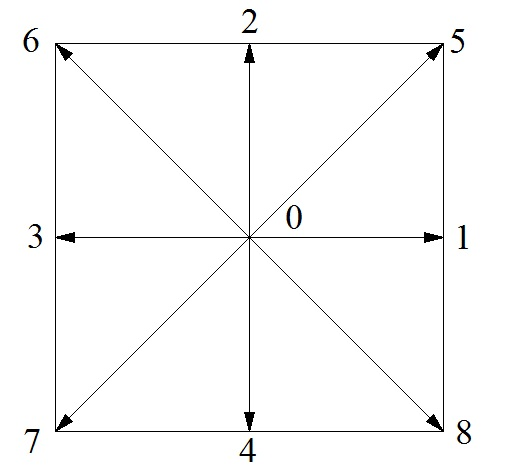
\includegraphics[width=0.6\textwidth]{d2q9.jpg}
\centering
\caption{D2Q9 lattice illustrating the discretization of space and velocity in two dimensions.}
\label{fig:d2q9}
\end{figure}

In order to solve Eq.~\eqref{eq:boltzmann_srt} numerically we must discretize in both space and time. We use a simple forward Euler scheme in time given by
\begin{equation}\label{eq:time_euler}
\frac{d}{dt} f(\bm{x}, \bm{v},t) \approx \frac{ f(\bm{x} +\bm{v}\delta t, \bm{v}, t + \delta t) - f(\bm{x}, \bm{v}, t)}{\delta t}
\end{equation}
where $\delta t$ is the size of a time step. We then discretized space into a lattice such as the one shown in Fig.~\ref{fig:d2q9}. Finally, we discretize velocity so that in one time step, traveling with discretized velocity $c_i$ returns us to one of the lattice nodes. The final distribution function propogation scheme can then be written as
\begin{equation}\label{eq:lattice_boltzmann_srt}
f(\bm{x} +\bm{c}_i\delta t, \bm{c}_i, t + \delta t) = f(\bm{x},\bm{c}_i,t) + \frac{\delta t}{\lambda} \left(f^{\mathrm{eq}}(\bm{x},\bm{c}_i) - f(\bm{x},\bm{c}_i, t)\right).
\end{equation}
This process is typically split into two steps called streaming and collision. Streaming moves the velocity populations along their velocity to a neighboring node and is the left term on the right hand side of Eq.~\eqref{eq:lattice_boltzmann_srt} while collision relaxes the populations towards the equilibrium state and is the right term on the right hand side. The macroscopic velocity can be computed at any lattice node and time with
\begin{equation}
\bm{u}(\bm{x},t) = \frac{1}{\rho} \sum_{i = 1}^{n} \bm{c}_i f(\bm{x},\bm{c}_i, t)
\end{equation}
where the sum runs over all of the discretized velocities in the stencil.

\textbf{TODO: Is below how it's implemented in walberla?}

Before moving on, we should say something about the form of the equilibrium distribution function (EDF). It is given by
\begin{equation}\label{eq:equilibrium_distribution_function}
f^{\mathrm{eq}}(\bm{x},\bm{c}_i,t) = f^{\mathrm{eq}}(\bm{u}(\bm{x},t),\bm{c}_i) \defeq\begin{cases}
\rho\lp1-\lp1-\omega_0\rp\frac{p}{\rho c_s^2}+s_0(\bm{u})\rp, & i = 0 \\
\rho\lp\omega_i\frac{p}{\rho c_s^2} + s_i(\bm{u})\rp, &\text{else}
\end{cases}
\end{equation}
where
\begin{equation}
s_i(\bm{u}) = \omega_i\lp\frac{\bm{c}_i\cdot \bm{u}}{c_s^2} + \frac{(\bm{c}_i \cdot \bm{u})^2}{2c_s^4} - \frac{\bm{u} \cdot \bm{u}}{2c_s^2}\rp,
\end{equation}
$c_s$ is the speed of sound, $p$, $\rho$, and $\bm{u}$ are the macroscopic pressure, density and velocity, and the $\omega_i$ are weights that depend on the lattice stencil.

\section{Oldroyd-B Algorithm}
Here we discuss the discretization of the constitutive equation. Recalling Eq.~\eqref{eq:full_oldroyd_b} we can split it into parts as
\begin{equation}\label{eq:oldroyd_b_operators}
\frac{\partial \bm{\tau}}{\partial t} + \bm{A}_{\mathrm{adv}}(\bm{\tau},t) =\bm{A}_{\mathrm{rel-str}}(\bm{\tau},t)
\end{equation}
where we have defined the advection and relaxation-stretching operators on $\bm{\tau}$ to be
\begin{equation}\label{eq:advection_operator}
\bm{A}_{\mathrm{adv}}(\bm{\tau},t) \defeq (\bm{u} \cdot \nabla)\bm{\tau},
\end{equation}
and
\begin{equation}\label{eq:relaxation_stretching_operator}
\bm{A}_{\mathrm{rel-str}}(\bm{\tau},t) \defeq \left(\bm{\tau} \cdot \nabla\bm{u} +(\nabla\bm{u})^T \cdot \bm{\tau}\right) + \frac{1}{\lambda_p}\left(2\eta_p \bm{d} - \bm{\tau}\right).
\end{equation}
We can directly calculate the relaxation-stretching operator by first computing the velocity field from the Lattice-Boltzmann distribution function. Derivatives are then taken using a two sided scheme as
\begin{equation}\label{eq:velocity_gradient_scheme}
(\nabla \bm{u})_{\alpha \beta} = \frac{\partial u_\beta}{\partial x_\alpha} = \frac{1}{2\delta x} \sum_{i=1}^{n}u_\beta(\bm{x} + \bm{c}_i\delta t, t)(\bm{c}_i)_\alpha
\end{equation}
where the $\alpha,\beta$ run over the number of dimensions and the sum runs over the \textit{cardinal} directions (extended with up and down for three dimensions).

We can avoid calculating the advection operator directly by exploiting the distribution function. Making use of the Einstein convention we can write Eq.~\eqref{eq:advection_operator} as
\begin{equation}\label{eq:advection_einstein_convention}
\bm{A}_{\mathrm{adv}}(\bm{\tau},t) = u_\alpha(\bm{x},t)\frac{\partial}{\partial x_\alpha} \bm{\tau}(\bm{x},t).
\end{equation}
Now the incompressible continuity equation states that
\begin{equation}\label{eq:continuity_einstein_convention}
\frac{\partial}{\partial x_\alpha} u_\alpha(\bm{x},t) = 0
\end{equation}
allowing us to rephrase Eq~\eqref{eq:advection_einstein_convention} as
\begin{equation}\label{eq:advection_intermediary}
\bm{A}_{\mathrm{adv}}(\bm{\tau},t) = \frac{\partial}{\partial x_\alpha}(\bm{\tau}(\bm{x},t)u_\alpha(\bm{x},t)).
\end{equation}
Now we can replace the velocity with its hydrodynamic mode to arrive at
\begin{equation}
\bm{A}_{\mathrm{adv}}(\bm{\tau},t) = \frac{1}{\rho} \frac{\partial}{\partial x_\alpha} \bm{\tau}(\bm{x},t)f(\bm{x},\bm{c}_i,t)(\bm{c}_i)_\alpha.
\end{equation}
We can truncate the Taylor expansion of this expression to arrive at the final form given by
\begin{multline}\label{eq:advection_full}
\bm{A}_{\mathrm{adv}}(\bm{\tau},t) = \frac{-1}{\rho \delta t}\left[2 \sum_{i=1}^n\bm{\tau}(\bm{x}-\bm{c}_i\delta t,t)f(\bm{x} - \bm{c}_i\delta t, \bm{c}_i,t)\right. \\
-1.5\sum_{i=1}^n\bm{\tau}(\bm{x},t)f(\bm{x}, \bm{c}_i,t) \\
\left.-0.5 \sum_{i=1}^n\bm{\tau}(\bm{x}-2\bm{c}_i\delta t,t)f(\bm{x} - 2\bm{c}_i\delta t, \bm{c}_i,t)\right]
\end{multline}
Finally, we can simply adopt a forward Euler scheme for the partial time derivative in Eq.~\eqref{eq:oldroyd_b_operators} which leaves us with the final form of the time evolution of the extra stress tensor as
\begin{equation}\label{eq:oldroyd_time_evolution}
\bm{\tau}(\bm{x},t+\Delta t) = \bm{\tau}(\bm{x},t) - \Delta t \bm{A}_{\mathrm{adv}}(\bm{\tau},t) + \Delta t \bm{A}_{\mathrm{rel-str}}(\bm{\tau},t)
\end{equation}
where the two operators are computed using Eqs.~\eqref{eq:advection_full} and \eqref{eq:relaxation_stretching_operator} respectively. Note that the Lattice-Boltzmann time step $\delta t$ and Oldroyd-B time step $\Delta t$ need not be the same.

\section{Coupling}
As seen in Eq.~\eqref{eq:momentum_conservation}, we couple the two types of equations through a force density calculated as the divergence of the extra stress tensor:
\begin{equation}
\bm{F} = \nabla \cdot \bm{\tau}
\end{equation}
We then calculate this divergence with a two sided derivative similarly to Eq.~\eqref{eq:velocity_gradient_scheme} given by
\begin{equation}\label{eq:divergence_scheme}
F_\alpha = \frac{1}{2\delta x}\sum_{i=1}^n\bm{\tau}(\bm{x}+\bm{c}_i\delta t,t)_{\beta \alpha}(\bm{c}_i)_\beta
\end{equation}
where again the $i$ run over only the cardinal directions. The $\beta$ here refer to the index of the $i$th direction, i.e. $0$ for east and west, $1$ for north and south, and $2$ for up and down and are not summed over. The above is simply a two side derivative form of 
\begin{equation}
(\nabla \cdot \bm{\tau})_\alpha = F_\alpha = \frac{\partial}{\partial x_\beta} \tau_{\beta \alpha} .
\end{equation}
This extra force manifests itself in the Lattice-Boltzmann method as an extra term on the right-hand side of the Lattice-Boltzmann equation~\eqref{eq:lattice_boltzmann_srt} leading to
\begin{equation}\label{eq:forced_lattice_boltzmann_srt}
f(\bm{x} +\bm{c}_i\delta t, \bm{c}_i, t + \delta t) = f(\bm{x},\bm{c}_i,t) + \frac{\delta t}{\lambda} \left(f^{\mathrm{eq}}(\bm{x},\bm{c}_i) - f(\bm{x},\bm{c}_i, t)\right) + \delta t F_i
\end{equation}
where
\begin{equation}
F_i = \omega_i \lp1-\frac{\delta t}{2 \lambda}\rp \lp \frac{\bm{c}_i - \bm{u}}{c_s^2} + \frac{(\bm{c}_i \cdot \bm{u})}{c_s^4}\bm{c}_i\rp\cdot\bm{F}
\end{equation}
and we now calculate macroscopic velocity as the average value before and after the force:
\begin{equation}\label{eq:forced_macroscopic_velocity} 
\rho\bm{u}(\bm{x},t) = \sum_{i=1}^n\bm{c}_i f(\bm{x},\bm{c}_i,t) + \frac{\delta t}{2} \bm{F}(\bm{x},t).
\end{equation}
The expression for macroscopic velocity above is now used for all other purposes including calculation of the EDF. We now have a fully coupled system of discretized equations and a well defined algorithm for developing them in time. 

\section{Boundary Conditions}

In order to model specific flow situations, we certainly must impose boundary conditions so that our simulated flows match external constraints. In this section we will touch on the handling of boundaries for both the Lattice-Boltzmann algorithm and for the Oldroyd-B algorithm.

\subsection{Periodic Boundary Conditions}

Probing systems which depend on the bulk properties of the fluid would require simulating an unreasonably large simulation box in order to nullify the effects of walls. The obvious solution is to use periodic boundary conditions (PBC) to allow some dimensions of our simulations to be effectively "infinite." This is simply implemented for both LB and Oldroyd-B by pulling values of the distribution function and stress tensor from the relevant domain node when crossing the PBC.

\subsection{No Slip Walls}
Important to the description of a physical hydrodynamic system is the concept of walls. In the context of the NS equations this clearly implies a boundary condition. Besides the obvious zero normal fluid velocity at walls, it is conventional to use a "no-slip" condition with zero fluid velocity tangential to the wall as well. In Lattice-Boltzmann, velocity boundary conditions are implemented using so-called bounce back boundary conditions. 

\textbf{TODO: Bounce back boundary conditions in LB}

Since we have fixed the velocity at the no-slip walls using the above, the Oldroyd-B algorithm will be responding to the correct velocity field. Moreover, there is no further constraint on the extra stress tensor at a wall. Walls do, however, introduce the idea of a valid domain for our algorithms which depend on neighboring values of the extra stress and distribution function. In order to avoid taking values from within walls we use the following advection operator in place of Eq.~\eqref{eq:advection_full} at nodes next to and one node removed from a wall node:
\begin{multline}\label{eq:near_boundary_advection_1}
\overset{\sim}{\bm{A}}_{\mathrm{adv}}(\bm{\tau},t)=  \frac{-1}{\rho \delta t}\left[\sum_{i=1}^n\bm{\tau}(\bm{x}-\bm{c}_i\delta t,t)f(\bm{x} - \bm{c}_i\delta t, \bm{c}_i,t)\right. \\
-\left.\sum_{i=1}^n\bm{\tau}(\bm{x},t)f(\bm{x}, \bm{c}_i,t)\right]
\end{multline}
where the tilde implies a modified operator near the boundary.

The above saves us from pulling values from walls when we are one node removed but not at the nearest neighbor points. In order to fix this we must use one sided calculations rather than two sided. There are three locations where the algorithm must be modified: the velocity gradient~\eqref{eq:velocity_gradient_scheme}, the stress divergence~\eqref{eq:divergence_scheme}, and the above advection operator~\eqref{eq:near_boundary_advection_1}.  We modify the velocity gradient as
\begin{equation}\label{eq:near_boundary_velocity_gradient}
\overset{\sim}{(\nabla \bm{u})}_{\alpha \beta} = \frac{1}{2\delta x} \sum_{i=1}^{n}\begin{cases} 
u_\beta(\bm{x} + \bm{c}_i\delta t, t)(\bm{c}_i)_\alpha, &  \bm{x} + \bm{c}_i \delta t \in \mathrm{domain}\\
2u_\beta(\bm{x}, t)(\bm{c}_i)_\alpha - u_\beta(\bm{x} - \bm{c}_i\delta t, t)(\bm{c}_i)_\alpha, & \mathrm{else}.
\end{cases}
\end{equation}
The stress divergence is similarly modified as
\begin{equation}\label{eq:near_boundary_stress_divergence}
\overset{\sim}{F}_\alpha = \frac{1}{2\delta x}\sum_{i=1}^n\begin{cases}
\bm{\tau}(\bm{x}+\bm{c}_i\delta t,t)_{\beta \alpha}(\bm{c}_i)_\beta, & \bm{x} + \bm{c}_i \delta t \in \mathrm{domain} \\
2\bm{\tau}(\bm{x},t)_{\beta \alpha}(\bm{c}_i)_\beta - \bm{\tau}(\bm{x}-\bm{c}_i\delta t,t)_{\beta \alpha}(\bm{c}_i)_\beta, & \mathrm{else}
\end{cases}
\end{equation}
and the advection operator becomes
\begin{multline}\label{eq:near_boundary_advection_2}
\overset{\sim}{\bm{A}}_{\mathrm{adv}}(\bm{\tau},t)=  \frac{-1}{\rho \delta t}\left[\sum_{i=1}^n\right.
\begin{cases}
\bm{\tau}(\bm{x}-\bm{c}_i\delta t,t)f(\bm{x} - \bm{c}_i\delta t, \bm{c}_i,t) , & \bm{x} - \bm{c}_i \delta t \in \mathrm{domain} \\
0, & \mathrm{else} 
\end{cases}\\
-\left.\sum_{i=1}^n\begin{cases}
\bm{\tau}(\bm{x},t)f(\bm{x}, \bm{c}_i,t), & \bm{x} + \bm{c}_i \delta t \in \mathrm{domain} \\
0, & \mathrm{else}\end{cases}\right]
\end{multline}
ensuring that there is no advection into or out of a boundary. The above algorithm fails in the case that there is one domain node between two boundary nodes but works in any other arbitrary geometry. 
\chapter{Benchmarks}
In the following, we present some results of benchmarks against which we tested our model. We have looked at two dimensional Poiseuille flow, the four roll mill, and plan to look at the lid driven cavity.

\section{Poiseuille Flow}
Poiseuille flow is a simple physical system which allows us to test how our algorithm treats boundaries and whether the paramaters available to us behave as expected. The physical model is fluid flow between two infinite parallel plates driven by either a pressure gradient or a homogeneous body force. We will use a body force to drive the fluid and the symmetry of the system will allow us to simulate in two dimensions. We take the periodic boundary conditions at the east and west boundaries and no slip walls on the north and south boundaries of the domain.





\section{Four Roll Mill}



\end{document}